\section{Implementation}
\label{sec:implementation}

\subsection{Framework Structure}

\begin{figure}
\centering
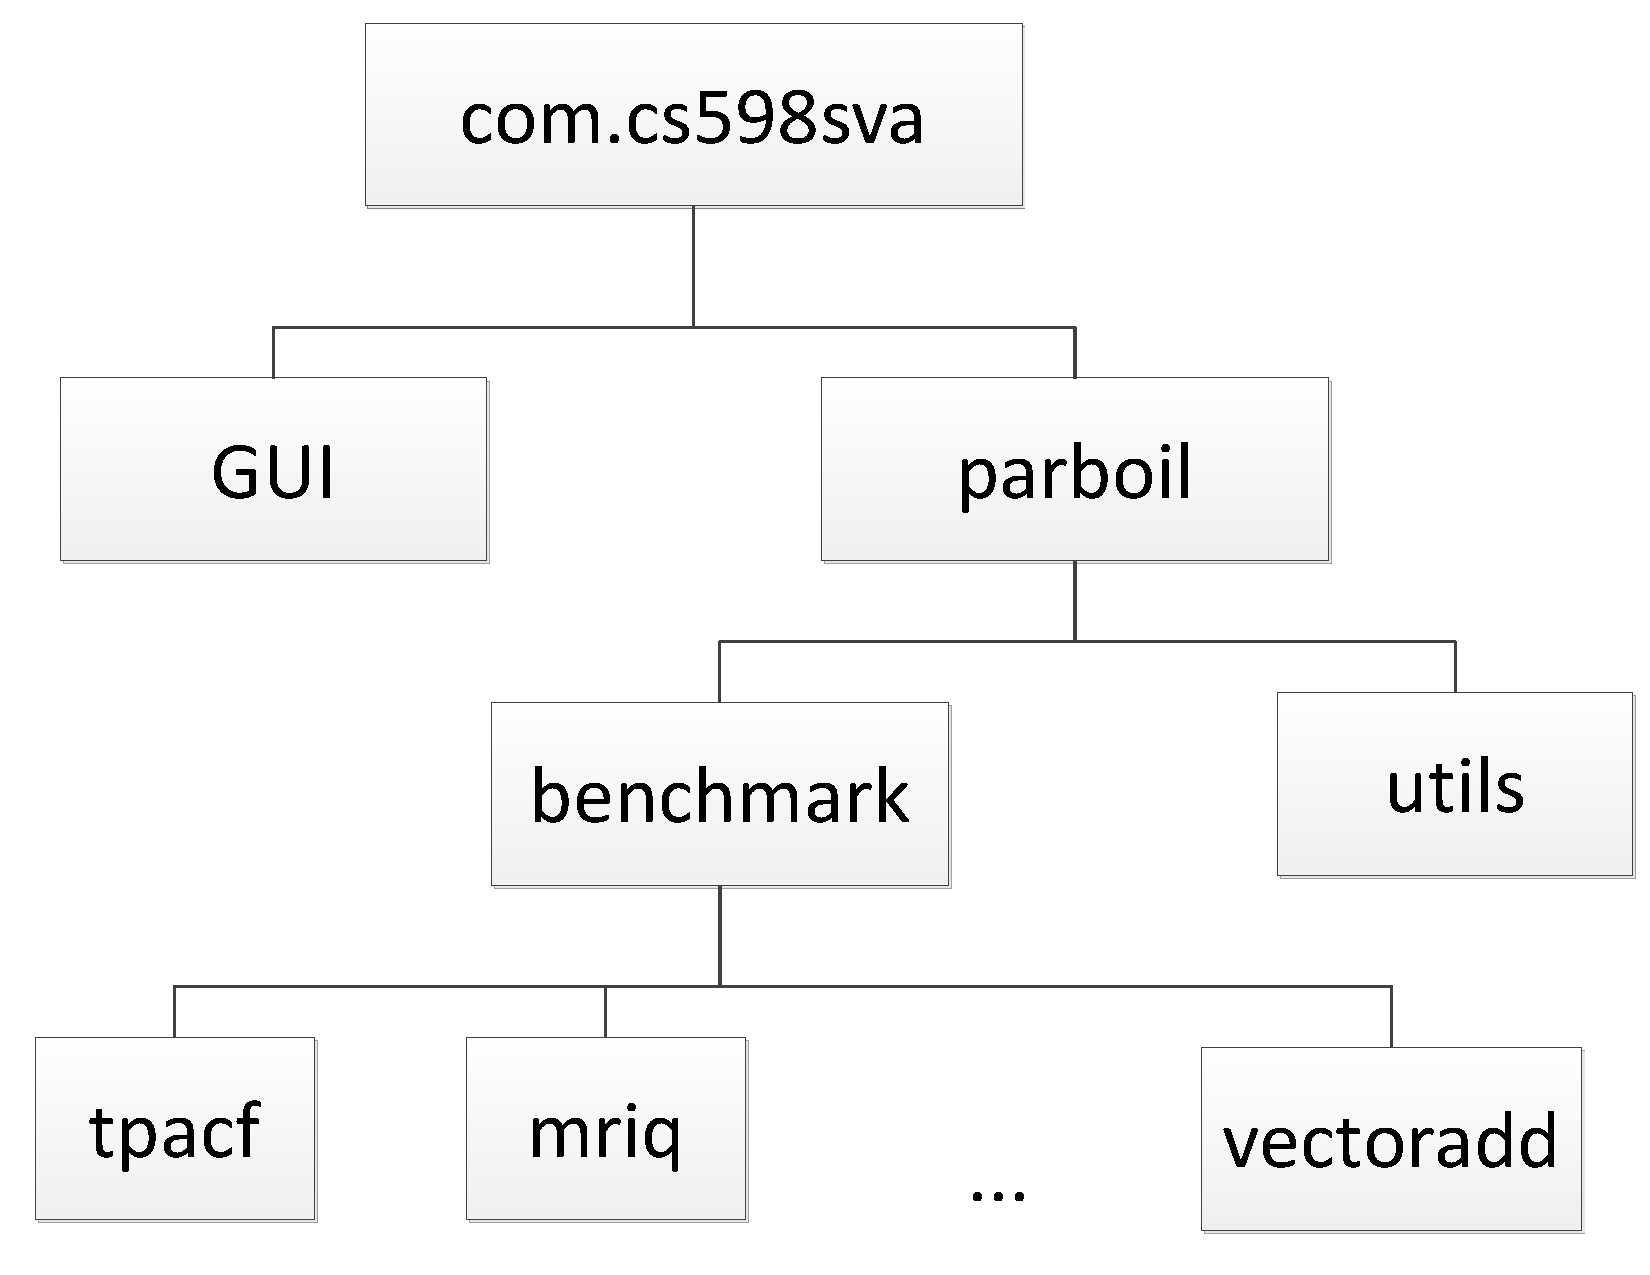
\includegraphics[scale=0.65]{figs/package_diagram.pdf}
\caption{The Java package structure.}
\label{fig:package_structure}
\centering
\end{figure}


\begin{figure}
\centering
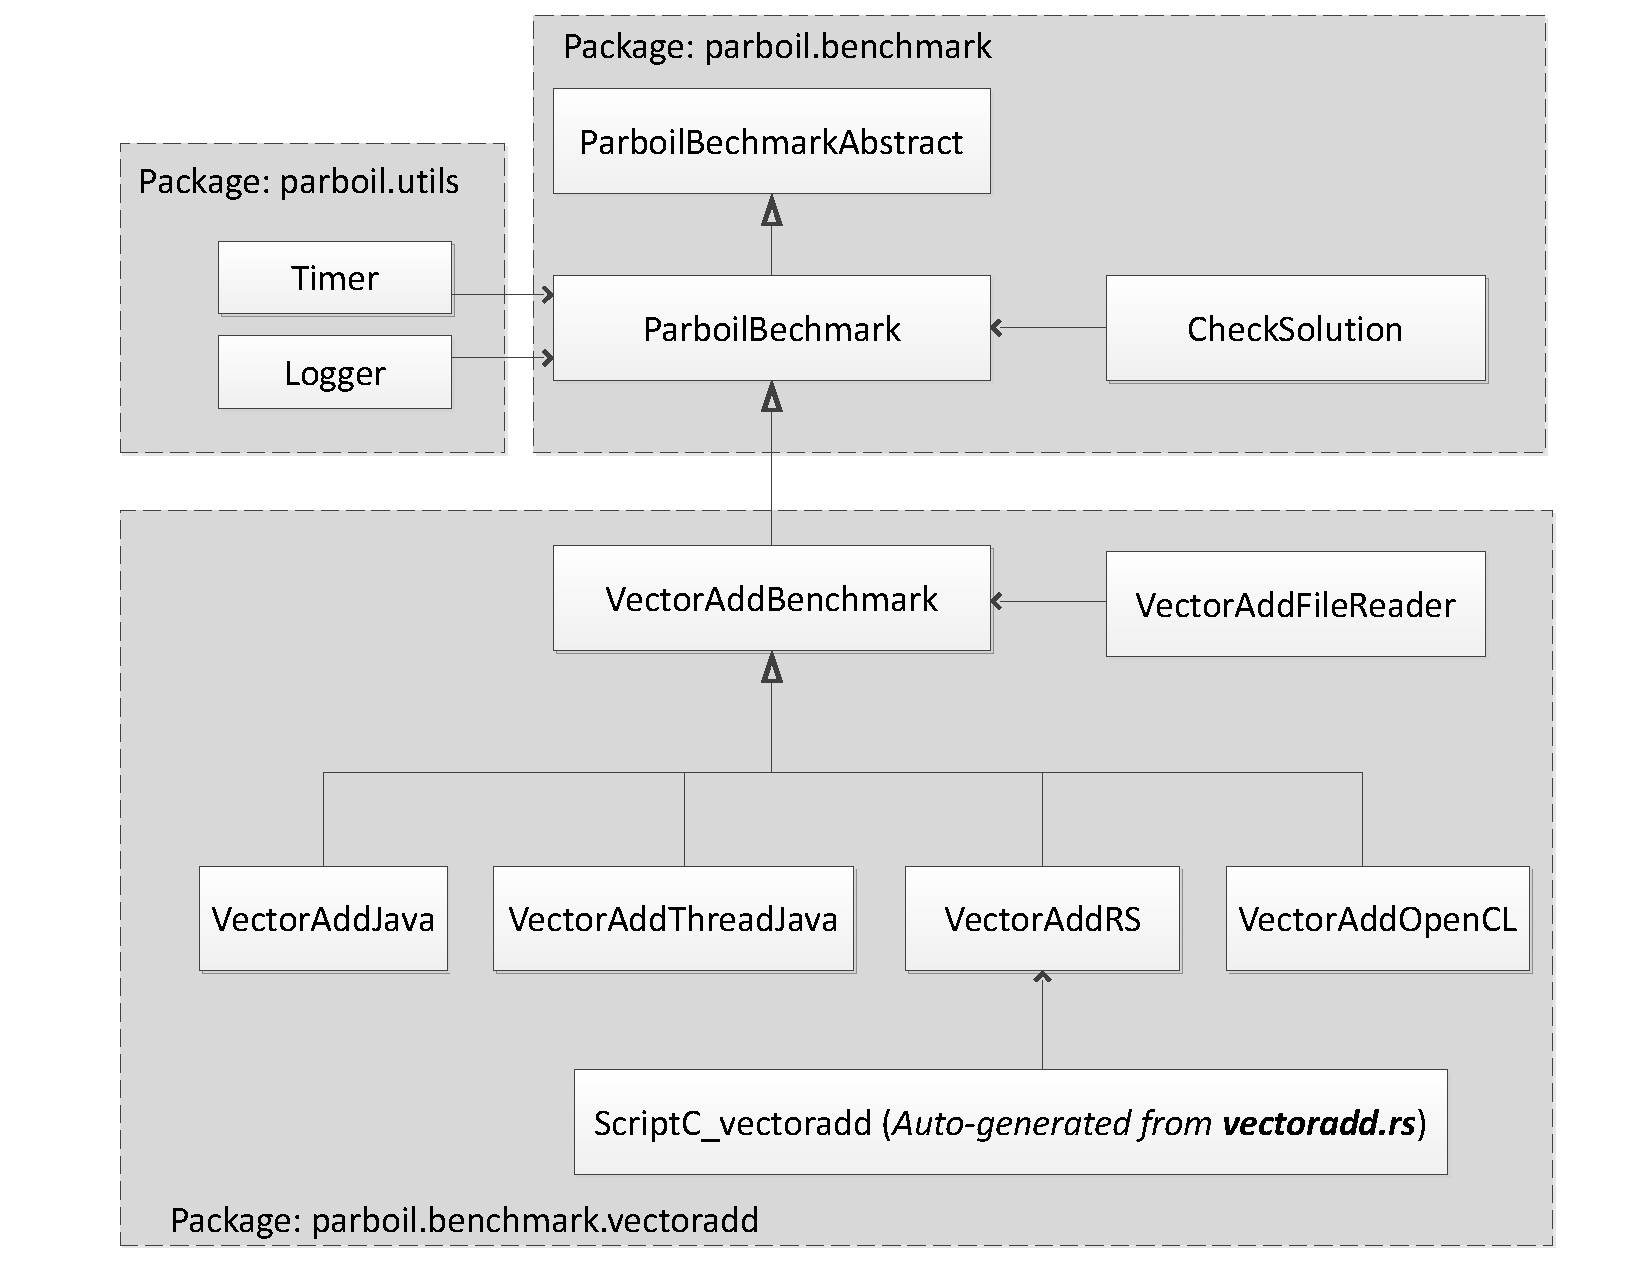
\includegraphics[scale=0.5]{figs/vectoradd_class_diagram.pdf}
\caption{Class diagram of the VectorAdd benchmark.}
\label{fig:class_diagram}
\centering
\end{figure}

In order to facilitate the development of the benchmarks, we designed a
framework,  which contains (i) a hierarchy of the benchmarks, e.g.,
all different implementations of the same benchmark are grouped together, and
(ii) utility functions that support measuring and recording the results.
Figure \ref{fig:package_structure} shows an overview of the framework by mean
of the Java package structure. Figure~\ref{fig:class_diagram} provides a closer
view at the organization of the classes related to the VectorAdd benchmark.

At a high level, we split the development of the graphical user interface (GUI),
from the development of each of the benchmarks, under the \fix{GUI} package and
the \fix{parboil} package in Figure~\ref{fig:package_structure}, respectively.
At this stage, the GUI is simply to allow users to start running the benchmarks,
and to display the status of the benchmark execution, e.g., in which stage a
benchmark is running, and whether a benchmark has executed successfully or
failed at the end. In the future, more features will be added, such as
displaying the final scores of the device.

The \fix{parboil} Java package is the core of the project. In this package, we
identified the common utility functions, such as timing- and logging-related
functions, that are used across all the benchmarks. Those functions are grouped
in classes, e.g., \fix{Timer} and \fix{Logger}, and implemented in the
\fix{utils} package. Each benchmark, e,g., \fix{TPACF} or \fix{Histogram}, is
implemented in a separate package under the \fix{benchmark} package. 

Figure~\ref{fig:class_diagram} shows the class diagram of the VectorAdd benchmark.
Other benchmarks have the same class structure. In order to implement a
benchmark, we just need to create a new class that inherits the \fix{ParboiBenchmark} class, which
layouts a common skeleton. For each benchmark, we have to implement a class to
read the input, for example the \fix{VectorAddFileReader} class in this case. Each
computational kernel, e.g., for Java, threaded Java, RenderScript, or OpenCL, is
implemented in a separate class, e.g., \fix{VectorAddJava},
\fix{VectorAddThreadedJava}, \fix{VectorAddRS}, or \fix{VectorAddOpenCL},
respectively. These classes inherit from the parent class of the benchmark ---
\fix{VectorAddBenchmark} in this case. This hierarchical design
maximizes the code reuse between benchmarks, and between computation kernels.  It
also allows for a consistent interface to run the benchmarks.


\subsection{Utility Functions}
\subsubsection{Timer}
The \fix{Timer} class is an important utility in our benchmark. It
determines the accuracy and flexibility of our measurement. The \fix{Timer}
class utilizes the Android's \fix{SystemClock}, which provides real-time clock at
nanosecond resolution. Each \fix{Timer} object consists of a dynamic list of
\fix{TimerElement} objects. Each \fix{TimerElement} object is a measure of a
particular execution segment, e.g., allocation time, setup time, and compute
time. In order to create a new \fix{TimerElement}, we just need to invoke the
\fix{Timer.start(category, message)} method at the beginning of the execution
segment we wish to measure (here category is a user defined category such as
``Compute'' or ``Setup'', while message is a message that further refines the
category such as ``Allocating temporary data structures''). At the end of the
execution segment, we need to invoke the \fix{Time.stop()} method. The
time-stamp and elapsed time will be automatically computed and recorded.
The \fix{Timer} class can also dump all the recorded \fix{TimerElement}s to a
SQLite database or serialize it to the JSON format for conveniently storing and
parsing the results.

If a benchmark is run multiple times, for example, we run the compute part 100
times for each small benchmark, and five times for each big benchmark in our
currently analysis, then the \fix{Timer} has a function to aggregate the results
to output the average time across runs.  Currently, we do not exercise that code
and we leave the statistical analysis to the parser and visualizer.

\subsubsection{Output to Database}

Unlike Parboil, which outputs the times to {\tt stdout}, we output our data into
a SQLite database.  This affords us a few things.  First, since data is
outputted in the specified columns, we do not have to re-parse the output data.
Second, timing information can be shared easily by copying the database.
Finally, we can store more than just timing information -- for example we also
store which machine the time has been taken on as well as which runtime is being
used.  Since writing to flash is expensive, all timing data is stored in memory,
and then after the benchmark has finished, it is inserted into the database. 

\subsubsection{Processor and Power Utilization}

Unlike programming desktops, where one mainly 
  improves software by increasing either features or performance,
  mobile programmers develop for increase features, performance, and 
  battery life.
In fact, one of the main selling points for heterogeneous
  programming on mobile devices, is the increase in battery life.
Increasingly, hardware vendors, such as Apple or Samsung, sell new
  mobile hardware by advertising longer battery life.
Finding a balance between energy consumption and performance is a 
  balancing act that a programmer would like to delegate to the 
  compiler or runtime.

Since Android does not offer a way to capture processor usage information
programmatically, we use the Trepn~\cite{profilerqualcomm} tool by Qualcomm to capture the data and save it into a {\tt csv} file.
This tool is limited to Qualcomm based
chipsets. Trepn reads internal processor counters as well as power rail information,
both of which are not available programmatically and are more accurate than reading
the information from the \fix{/proc} kernel file system.

Trepn is an external application that is run outside of our benchmark framework.
To pass messages to Trepn, we make use of Android's \fix{Intent} framework.
The \fix{Intent} framework allows one to pass messages between applications.
Trepn records the time a message is received (which corresponds to time blocks
in our code) and we developed scripts to correlate Trepn's data dump with both
the load and power usage.

We set Trepn to read
the counters every $100ms$ and measure the load and power usage separately to
decrease the overhead of the profiler.  To reduce overhead, Trepn measures the
processor usage information every $100ms$, both the frequency and the load are
measured sequentially, we therefore needed to correct that when parsing the {\tt
csv} file.

First, we parse each processor reading along with the time-stamps for reading the
file.  Next, we interpolate the measured data (we use linear interpolation), and
evaluate the interpolated value at the application state times (these are the times
Trepn received signals from our application and correspond to timed blocks of
code).  We then multiply the load by the frequency, and rescale all the CPU and
GPU data (we perform the rescaling on the CPU and GPU separately).  Trepn can
have measurement errors, resulting in infinite numbers.  To make sure that these
do not skew the plots, we clip the range of possible processor reading to be
between 1 and $0.99$th quantile of the data.  While efforts have
been taken to reduce the profiler's overhead, the overhead is still around
$10\%$.


\subsection{Implementing Computational Kernels}
\label{sec:implementationRS}

\begin{table}
\centering
\begin{tabu} to \textwidth { | l | c |}
    \hline 
    Language      & Line Count \\ \hline
    Java          & 7549       \\ \hline
    RenderScript  & 1000       \\ \hline
    JNI/C++       & 2048       \\ \hline
    OpenCL        & 480        \\ \hline
\end{tabu}
\caption{RSBench project line count breakdown.}
\label{table:breakdown}
\end{table}

Table~\ref{table:breakdown} shows the numbers of line-of-code (LOC) broken down
into different types of programming languages in the RSBench project. The next
sub-sections describe the process of implementing different types of computational
kernels for each benchmark.

\subsubsection{RenderScript Kernels}
%This section describes the general steps to write a computation kernel in
%RenderScript for our benchmark.

By design, each RenderScript kernel produces an \textit{element} of the output.
It is up to developers to define the granularity of an element. For example, in
the VectorAdd benchmark, an output element can be one, or two, or three array
elements of the output vector. This granularity essentially determines the
parallelism of the written RenderScript code. In our benchmarks, we select the
finest granularity of the output element, e.g., one array element in this case,
to implement our RenderScript kernel.

In order to support this model, the RenderScript framework provides APIs to (i)
define the type of \fix{Element} for both input and output of RenderScript
kernels, and (ii) pack \fix{Element}s into \fix{Allocation}, which is the data
structure that is used to pass data back and forth between regular Java code and
RenderScript code.

A significant effort of our work is to determine efficient ways to convert input
data from original structure to the \fix{Allocation} structure with appropriate
\fix{Element} type. This conversion is also reflected at runtime through the
\textit{setup} time category of RenderScript execution.

After data has been packed into \fix{Allocation} objects, we move to write
RenderScript code in the C99 format. The code needs to be placed in a specific file
with the $.rs$ extension and a proper header, so that the Android Development
Tools (ADT) can automatically generate a wrapper Java class for it. The
auto-generated Java class provides interfaces to invoke the RenderScript code
from Java code.

The RenderScript targets the $4.3$ and $4.4$ Android platforms and 
	is compiled with \fix{renderscript.support.mode=false} which
	allows the compiler to use some optimizations which were not available in
	previous Android versions.

\subsubsection{Native Kernels}

Android applications are hosted with Dalvik VM and therefore native code
	--- C, OpenMP, and OpenCL --- has to be invoked through Java Native
	Interface (JNI). 
	Aside from
wrapping the code via JNI so it is callable from within Java, little
modification was done to the Parboil version of the C and OpenMP code.


The OpenCL kernels are lifted from Parboil as well, but we rewrite the 
	OpenCL host code using the C++ OpenCL API, since it simplifies some of the
	code and affords more code reuse opportunities.
We use the \fix{base} implementation of OpenCL --- this a
platform agnostic unoptimized implementation.

To allow devices with no OpenCL support to make use of the C and OpenMP
implementations, we generate 3 libraries (one for C, OpenMP, and OpenCL).  Each
library is then loaded and called from with its class implementation.
The \fix{-O3 -ftree-vectorize -mvectorize-with-neon-quad}
 compile option  is set when compiling the libraries, this allows the compiler the opportunity to autovectorization code.
